\documentclass[a4paper,12pt]{article}
\usepackage[utf8]{inputenc}
\usepackage[spanish]{babel}
\usepackage{color}
\usepackage{parskip}
\usepackage{graphicx}
\usepackage{multirow}
\usepackage{listings}
\usepackage{vmargin}
\graphicspath{ {imagenes/} }
\definecolor{mygreen}{rgb}{0,0.6,0}
\definecolor{lbcolor}{rgb}{0.9,0.9,0.9}
\usepackage{epstopdf}


\setpapersize{A4}
\setmargins{2.5cm}       % margen izquierdo
{1.5cm}                        % margen superior
{16.5cm}                      % anchura del texto
{23.42cm}                    % altura del teAxto
{10pt}                           % altura de los encabezados
{1cm}                           % espacio entre el texto y los encabezados
{0pt}                             % altura del pie de página
{2cm}     

\lstset{
backgroundcolor=\color{lbcolor},
    tabsize=4,    
%   rulecolor=,
    language=[GNU]C++,
        basicstyle=\tiny,
        aboveskip={1.5\baselineskip},
        columns=fixed,
        showstringspaces=false,
        extendedchars=false,
        breaklines=true,
        prebreak = \raisebox{0ex}[0ex][0ex]{\ensuremath{\hookleftarrow}},
        frame=single,
        showtabs=false,
        showspaces=false,
        showstringspaces=false,
        identifierstyle=\ttfamily,
        keywordstyle=\color[rgb]{0,0,1},
        commentstyle=\color[rgb]{0.026,0.112,0.095},
        stringstyle=\color{red},
        numberstyle=\color[rgb]{0.205, 0.142, 0.73},
%        \lstdefinestyle{C++}{language=C++,style=numbers}’.
}

\begin{document}
  \twocolumn[
 \section{Problema}
 Implementar las operaciones insert y delete de un BST (Binary Search Tree).\\]
 \section{Código}
 \subsection{Tree.h}
 \begin{lstlisting}
#include "list"
#include "algorithm"
#include "fstream"

using namespace std;

template <typename T>
class Tree
{
    public:
        Tree();
        class Nodo{
            public:
                Nodo();
                Nodo(T dato);
                T dato;
                Nodo * hijos[2];
                void destruir();
        };
        bool find(T, Nodo **&);
        bool insert(T dato);
        void del(T valor);
        virtual ~Tree();
        void printDot();
    protected:
    private:
        void _menorIzq(Nodo **&);
        Nodo * root;
};
template <typename T>
bool Tree<T>::insert(T dato){
    Nodo **nodo;
    if(find(dato,nodo))return false;
    *nodo = new Nodo(dato);
    return true;
}

template <typename T>
bool Tree<T>::find(T dato, Nodo **&nodo){
    nodo = &root;
    while(*nodo != nullptr){
        if((*nodo)->dato == dato)return true;
        nodo = &((*nodo)->hijos[(*nodo)->dato < dato]);
    }
    return false;
}
template <typename T>
void Tree<T>::_menorIzq(Nodo ** &nodo){
    nodo = &((*nodo)->hijos[0]);
    while(true){
        if(!(*nodo)->hijos[1])return;
        nodo = &((*nodo)->hijos[1]);
    }
}
template <typename T>
void Tree<T>::del(T valor){
    Nodo ** nodo;
    if(!this->find(valor,nodo))return;
    if((*nodo)->hijos[0] and (*nodo)->hijos[1]){
        Nodo ** temp = nodo;
        _menorIzq(temp);
        swap((*temp)->dato, (*nodo)->dato);
        nodo = temp;
    }
    if((*nodo)->hijos[0]){
        *nodo = (*nodo)->hijos[0];
    }
    else if((*nodo)->hijos[1]){
        *nodo = (*nodo)->hijos[1];
    }
    else{
        *nodo = nullptr;
    }
}
template <typename T>
void Tree<T>::printDot(){
    ofstream archivo("eje.dot");
    if(archivo.fail()){
        cout<<"EL archivo no se pudo abrir"<<endl;
        return;
    }
    archivo<<"digraph{";
    list<Nodo *> result;
    if(root) result.push_back(root);
    for(auto iter = result.begin(); iter != result.end(); ++iter){
        archivo<<(*iter)->dato<<endl;
        if((*iter)->hijos[0]){
            archivo<<(*iter)->dato<<"->"<<(*iter)->hijos[0]->dato<<endl;
            result.push_back((*iter)->hijos[0]);
        }
        if((*iter)->hijos[1]){
            archivo<<(*iter)->dato<<"->"<<(*iter)->hijos[1]->dato<<endl;
            result.push_back((*iter)->hijos[1]);
        }
    }
    archivo<<"}";
    archivo.close();
    system("dot -Tpdf eje.dot -o eje.pdf");
}
template <typename T>
void Tree<T>::Nodo::destruir(){
    if(hijos[0])hijos[0]->destruir();
    if(hijos[1])hijos[1]->destruir();
    delete this;
}
template <typename T>
Tree<T>::Tree(){
    root = nullptr;
}

template <typename T>
Tree<T>::Nodo::Nodo(){
    hijos[0] = nullptr;
    hijos[2] = nullptr;
}

template <typename T>
Tree<T>::Nodo::Nodo(T dato){
    this->dato = dato;
    hijos[0] = nullptr;
    hijos[1] = nullptr;
}

template <typename T>
Tree<T>::~Tree(){
    if(root) root->destruir();
}
\end{lstlisting}
La funcion printDot es usada para generar un pdf con el arbol dibujado. Para esto utilizo un software llamado graphviz. Creamos un archivo .dot y luego ejecutamos una linea de comando para generar el respectivo pdf.
Esta funcion la usaremos para visulizar los ejemplos.
\newpage
\subsection{main.cpp}
\begin{lstlisting}
#include <iostream>
#include "Tree.h"

using namespace std;

int main()
{
    Tree<int> arbolito;
    arbolito.insert(9);
    arbolito.insert(5);
    arbolito.insert(14);
    arbolito.insert(3);
    arbolito.insert(8);
    arbolito.insert(11);
    arbolito.insert(20);
    arbolito.insert(16);
    arbolito.insert(18);
    arbolito.printDot();
    arbolito.del(18);
    arbolito.del(14);
    arbolito.del(20);
    arbolito.printDot();
}
\end{lstlisting}
\section{Ejemplos}
Los archivos .dot tienen una determinada estructura. Todo se escribe dentro de 'digraph{}'.
El archivo .dot que se genera al usar por primera vez la funcion 'printDot' es el siguiente:
\begin{lstlisting}
digraph{
9
9->5
9->14
5
5->3
5->8
14
14->11
14->20
3
8
11
20
20->16
16
16->18
18
}
\end{lstlisting}
Los nodos se escriben solos para inicializarlos para luego poder crear sus relaciones con el operador '-$>$'.
\begin{figure}[h]
 \centering
 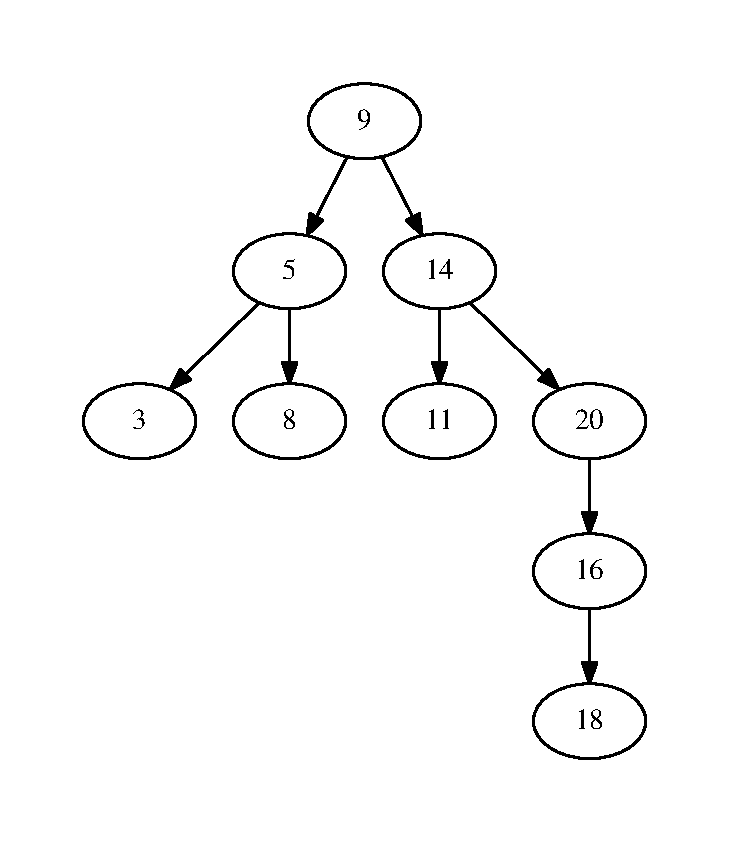
\includegraphics[scale = 0.5]{1.pdf}
 \caption{Imagen antes del delete}
\end{figure}
\begin{figure}[h]
 \centering
 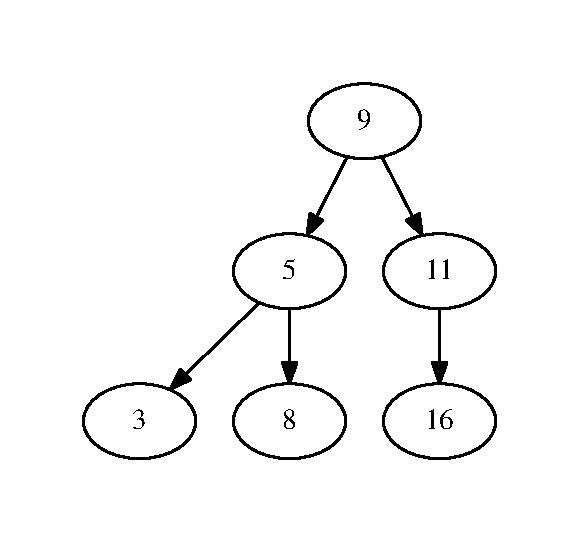
\includegraphics[scale = 0.5]{2.pdf}
 \caption{Imagen despues del delete}
\end{figure}

\end{document}
